\documentclass[a4paper, 12pt]{amsart}
\usepackage[french]{babel}
\usepackage[utf8]{inputenc}
\usepackage{amssymb}
\usepackage{graphicx}
\usepackage{coursebook}
\fthmstyle{plain}
\newfancythm{fthm}{Théorème}
\fthmstyle{defn}
\newfancythm{fdefn}{Définition}
\fthmstyle{ex}
\newfancythm{fex}{Exercice}
%\DeclareMathOperator*{\ln}{ln}
\newcommand{\pd}[2]{\ensuremath{\frac{\partial #1}{\partial #2}}}
\usepackage{pgf,tikz}
\usetikzlibrary{arrows, shapes}
\usetikzlibrary[patterns]
\usetikzlibrary{calc,fadings,decorations.pathreplacing, bending} 
\usetikzlibrary{decorations.markings}
\usetikzlibrary{decorations.pathmorphing}
\usetikzlibrary{positioning}
\usetikzlibrary{intersections}
\usetikzlibrary{hobby}

\title{Exercices - thème résidus et transformée de Laplace}
\setcounter{section}{5}
\graphicspath{{../images}}
\begin{document}
\maketitle
\begin{fex} 
    Calculer les trois premiers termes non nuls du développement en série de Laurent de $\cot z$ au voisinage de l'origine.
\end{fex} 
On a:
\[
\begin{split}
    & \sin(z) = \sum_{n\geq 0} (-1)^n \frac{z^{2n+1}}{(2n+1)!} \\
     & \cos(z) = \sum_{n\geq 0} (-1)^n \frac{z^{2n}}{(2n)!}
\end{split}
\]
En appliquant l'algorithme de division selon les puissances croissantes, il vient:
\[
\frac{\cos z}{\sin z} = \frac{1}{z} - \frac{z}{3} - \frac{z^3}{45}
\]
\begin{fex} 
On veut déterminer l'original de l'application~:
\[
F : p \to \frac{1}{1+p^3}
\]
\begin{itemize} 
\item Calculer, en précisant l'abscisse de convergence, la transformée de Laplace de l'application:
\[
f \colon t \mapsto \begin{cases}
    0 & t< 0 \\
    e^{-at} & t \geq 0, a \in \C
\end{cases}
\]
\item Décomposer $F$ en éléments simples et en déduire son original $f.$
\item Retrouver ce résultat par la formule d'inversion de Mellin-Fourier.
\end{itemize} 
\end{fex} 
Une primitive de l'application $t \mapsto e^{-(a+p)t}$ est:
\[
-\frac{e^{-(a+p)t}}{p+a}
\]
On en déduit que l'intégrale de Laplace:
\[
\int_0^{+\infty} e^{-(a+p)t} dt
\]
est convergente si et seulement si $\Re{p}> -\Re{a}.$
Elle vaut alors:
\[
\mathcal{L}(f)(p) = \frac{1}{p+a}
\]
La décomposition en éléments simples de $F$ est:
\[
\frac{1}{1+p^3} = \frac{1}{3} \frac{1}{1+p}
+\frac{e^{-i 2 \pi /3}}{3}\frac{1}{1-e^{i\pi /3}} 
+\frac{e^{i 2 \pi /3}}{3}\frac{1}{1-e^{-i \pi /3}}
\]
L'original de $F$ est donc, après simplification:
\[
\frac{1}{3} e^{-t} \left(1+\sqrt{3} e^{\frac{3 t}{2}} \sin \left(\frac{\sqrt{3} t}{2}\right) -e^{\frac{3 t}{2}} \cos \left(\frac{\sqrt{3} t}{2}\right)\right)
\]

On remarque tout d'abord que les coefficients de la décomposition en éléments simples sont les résidus de $F$ sur les trois points singuliers $-1,e^{i \pi/3},e^{-i \pi /3}.$ On intègre sur le contour \ref{fig:contour_laplace}:
\begin{figure}
    \centering
    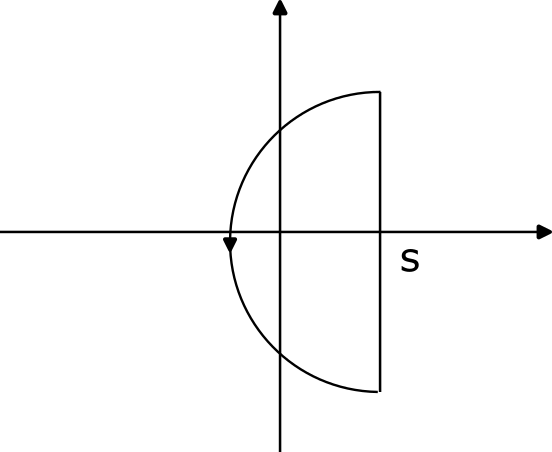
\includegraphics{contour_laplace.png}
    \caption{Contour pour Mellin-Fourier.}
    \label{fig:contour_laplace}
\end{figure}
avec $s > 1/2$, par exemple $s=1.$
Sur le demi-cercle de rayon $R > 2$, on majore l'intégrale par l'inégalité ML, soit:
\[
\pi \frac{R}{R^3-2} 
\]
qui admet pour limite $0$ lorsque $R$ tend vers $+\infty$.
On conclut alors par la formule d'inversion de Mellin-Fourier.
\end{document} 
\end{document}